\documentclass{article}

% if you need to pass options to natbib, use, e.g.:
%     \PassOptionsToPackage{numbers, compress}{natbib}
% before loading neurips_2018

% ready for submission
% \usepackage{neurips_2018}

% to compile a preprint version, e.g., for submission to arXiv, add add the
% [preprint] option:
     \usepackage[preprint]{nips_2018}

% to compile a camera-ready version, add the [final] option, e.g.:
%     \usepackage[final]{nips_2018}

% to avoid loading the natbib package, add option nonatbib:
%     \usepackage[nonatbib]{neurips_2018}

\usepackage[utf8]{inputenc} % allow utf-8 input
\usepackage[T1]{fontenc}    % use 8-bit T1 fonts
\usepackage{hyperref}       % hyperlinks
\usepackage{url}            % simple URL typesetting
\usepackage{booktabs}       % professional-quality tables
\usepackage{amsfonts}       % blackboard math symbols
\usepackage{nicefrac}       % compact symbols for 1/2, etc.
\usepackage{microtype}      % microtypography
\usepackage{packages}
\newcommand{\pfrac}[2]{\frac{\partial #1}{\partial #2}}

\title{Deep Learning Assignment 1}

\author{%
  Jochem Loedeman \\
  12995282
}

\begin{document}

\maketitle


\section{MLP backprop and NumPy Implementation}
\subsection{Evaluating the Gradients}
\subsubsection*{Question 1.1}
\begin{enumerate}[label=(\alph*)]
	\item 
	Given that
	$$
	\b Y = \b X \b W^T + \b B,
	$$ we deduce that
	$$
	Y_{mn} = \sum_p X_{mp}W_{np} + B_{mn}.
	$$ We will now find the required derivatives.
	\begin{enumerate}[label=(\roman*)]
	\item 
	$$
	\begin{aligned}
	\pfrac{L}{W_{ij}} &= \sum_{m, n}\pfrac{L}{Y_{mn}}\pfrac{Y_{mn}}{W_{ij}}.
	\end{aligned}
	$$ But
	$$
	\begin{aligned}
	\pfrac{Y_{mn}}{W_{ij}} &= \sum_pX_{mp}\pfrac{W_{np}}{W_{ij}} = \sum_pX_{mp}\delta_{ni}\delta_{pj} = X_{mj}\delta_{ni},
	\end{aligned}
	$$ and hence
	$$
	\begin{aligned}
	\pfrac{L}{W_{ij}} &= \sum_{m, n}\pfrac{L}{Y_{mn}}X_{mj}\delta_{ni} = \sum_m \pfrac{L}{Y_{mi}}X_{mj}.
	\end{aligned}
	$$ In matrix-vector notation, this is equivalent to
	$$
	\pfrac{L}{\b W} = \left(\pfrac{L}{\b Y}\right)^T\b X
	$$
	\item
	$$
	\pfrac{L}{b_i} = \sum_{m, n}\pfrac{L}{Y_{mn}}\pfrac{Y_{mn}}{b_i}
	$$
	But
	$$
	\pfrac{Y_{mn}}{b_i} = \pfrac{B_{mn}}{b_i} = \delta_{ni},
	$$ Since $B_{mn} = b_n$ for all $m = 1,\dots, S$. Therefore,
	$$
	\pfrac{L}{b_i} = \sum_{m, n}\pfrac{L}{Y_{mn}}\delta_{ni} = \sum_{m}\pfrac{L}{Y_{mi}}.
	$$ In matrix-vector notation, this is equivalent to
	$$
	\pfrac{L}{\b b} = \b 1 \pfrac{L}{\b Y}
	$$ where $\b 1$ is the $1 \times S$ ones-vector.
	\item 
	$$
	\pfrac{L}{X_{ij}} = \sum_{m, n}\pfrac{L}{Y_{mn}}\pfrac{Y_{mn}}{X_{ij}}.
	$$ But
	$$
	\pfrac{Y_{mn}}{X_{ij}} = \sum_p\pfrac{X_{mp}}{X_{ij}}W_{np} = \sum_p\delta_{mi}\delta_{pj}W_{np} = \delta_{mi}W_{nj},
	$$
	so
	$$
	\pfrac{L}{X_{ij}} = \sum_{m, n}\pfrac{L}{Y_{mn}}\delta_{mi}W_{nj} = \sum_n \pfrac{L}{Y_{in}}W_{nj}.
	$$ In matrix-vector notation, this is equivalent to
	$$
	\pfrac{L}{\b X} = \pfrac{L}{\b Y}\b W
	$$
\end{enumerate}
	\item Like before, we have
	$$
	\pfrac{L}{X_{ij}} = \sum_{m, n}\pfrac{L}{Y_{mn}}\pfrac{Y_{mn}}{X_{ij}}
	$$ But
	$$
	\pfrac{Y_{mn}}{X_{ij}} = \pfrac{h(X_{mn})}{X_{ij}} = h'(X_{mn})\delta_{mi}\delta_{nj},
	$$ and therefore,
	$$
	\pfrac{L}{X_{ij}} = \sum_{m, n}\pfrac{L}{Y_{mn}}h'(X_{mn})\delta_{mi}\delta_{nj} = \pfrac{L}{Y_{ij}}h'(X_{ij}).
	$$ Or, in matrix-vector notation:
	$$\pfrac{L}{\b X} = \pfrac{L}{\b Y} \circ h'(\b X)$$
	\item
	\begin{enumerate}[label=(\roman*)]
		\item
		$$
		 \pfrac{L}{X_{ij}} = \sum_{m, n}\pfrac{L}{Y_{mn}}\pfrac{Y_{mn}}{X_{ij}}.
		$$ The derivative of the softmax is
		$$
		\begin{aligned}
		\pfrac{Y_{mn}}{X_{ij}} &= \pfrac{}{X_{ij}} \frac{e^{X_{mn}}}{\sum_ke^{X_{mk}}} \\ &= \frac{\sum_ke^{X_{mk}} \cdot e^{X_{mn}}\delta_{mi}\delta_{nj} - e^{X_{mn}}\cdot\sum_ke^{X_{mk}}\delta_{mi}\delta_{kj}}{\left(\sum_ke^{X_{mk}}\right)^2} \\ &= \frac{\sum_ke^{X_{mk}} \cdot e^{X_{mn}}\delta_{mi}\delta_{nj} - e^{X_{mn}}\cdot e^{X_{mj}}\delta_{mi}}{\left(\sum_ke^{X_{mk}}\right)^2}\\
		&= Y_{mn}\delta_{mi}\delta_{nj} - Y_{mn}Y_{mj}\delta_{mi} \\ &= Y_{mn}\delta_{mi}\left(\delta_{nj} - Y_{mj}\right)
		\end{aligned}
		$$ Notice that when $m = i$ (i.e. when the same data point is considered), the derivative reduces to the usual softmax derivative for rank-1 tensors.
		
		We get
		$$
		\begin{aligned}
		\pfrac{L}{X_{ij}} &= \sum_{m, n}\pfrac{L}{Y_{mn}}Y_{mn}\delta_{mi}\left(\delta_{nj} - Y_{mj}\right) \\ &= \sum_n\pfrac{L}{Y_{in}}Y_{in}\left(\delta_{nj} - Y_{ij}\right)
		\end{aligned}
		$$
		\item 
		$$
		\begin{aligned}
		\pfrac{L}{X_{ij}} &= -\frac{1}{S}\sum_{m, n}T_{mn}\pfrac{\log X_{mn}}{X_{ij} }\\ &= -\frac{1}{S}\sum_{m, n}\frac{T_{mn}}{X_{mn}}\pfrac{X_{mn}}{X_{ij}} \\ &= -\frac{1}{S}\sum_{m, n}\frac{T_{mn}}{X_{mn}}\delta_{mi}\delta_{nj} \\ &= -\frac{1}{S}\frac{T_{ij}}{X_{ij}}
		\end{aligned}
		$$ The equation can be vectorized by using the elementwise division operator, known as the Hadamard division.
		$$
		\pfrac{L}{\b X} = -\frac{1}{S} \; \b T \oslash \b X
		$$
	\end{enumerate}
\end{enumerate}
\subsection{NumPy Implementation}
\subsubsection*{Question 1.2}
Training and testing the network for the default parameters, the following loss and accuracy curves as shown in Figure \ref{fig:npcurves} were obtained. Note that the losses are with respect to the training set, whereas the accuracy is obtained from the test set. The classifier reaches an asymptotic accuracy of approximately $0.48$.
\begin{figure}[H]
	\centering
	\subfloat[]{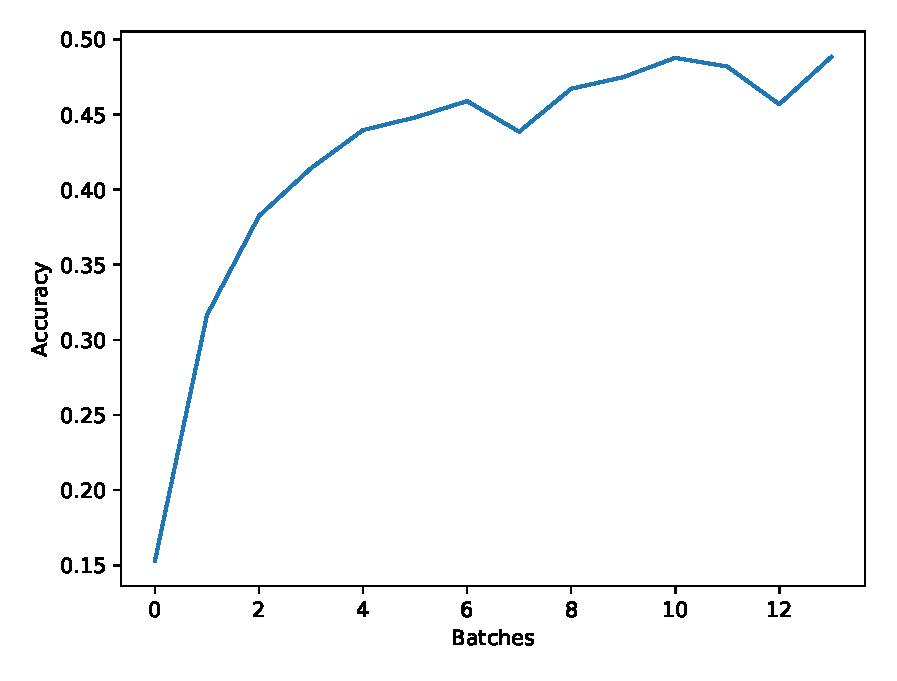
\includegraphics[width=.5\textwidth]{numpyAccuracy.eps}}
	\subfloat[]{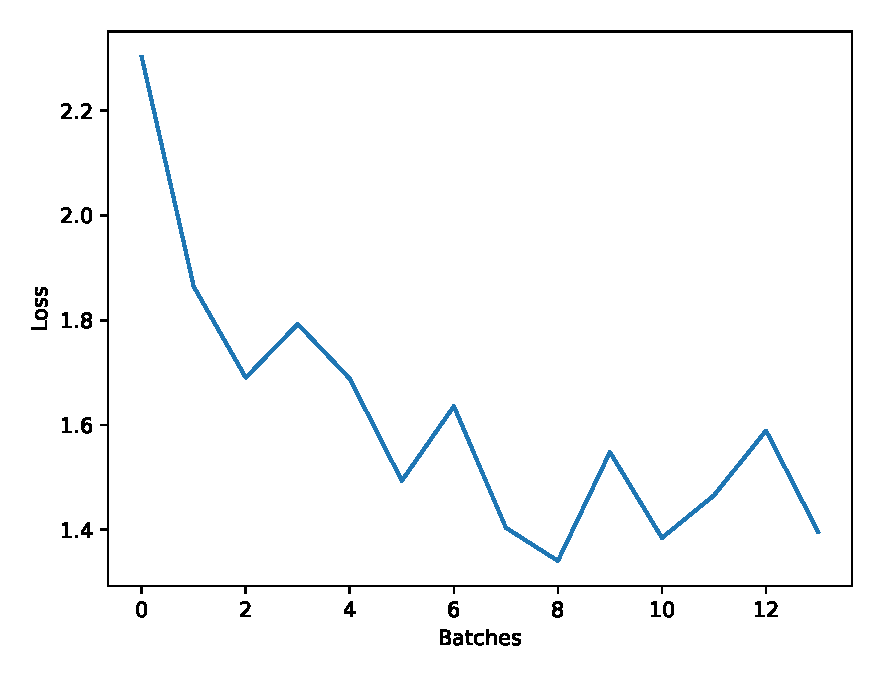
\includegraphics[width=.5\textwidth]{numpyLoss.eps}}
	\caption{Accuracy and loss for the NumPy implementation of the MLP}
	\label{fig:npcurves}
\end{figure}
\section{PyTorch MLP}
\subsubsection*{Question 2.1}
Next, the same MLP was implemented using PyTorch. With the default parameters, an accuracy of 0.48 was reached. The following changes were made to the default network to increase the performance:
\begin{itemize}
	\item A second layer, also consisting of $100$ units was added. This modification in itself did not increase the accuracy. However, together with the next modification in this list, it increased accuracy with $0.02$.
	\item The larger network needed more iterations for the accuracy to converge, so the maximum number of steps was increased to $3000$. It led to another accuracy gain of $0.02$.
	\item The optimizer was changed to Adam. Without this modification, the others seem to have much less effect. Changing from SGD to Adam with the other modifications in place, the accuracy increase is $0.07$. Adam improves on regular SGD by including an adaptive learning rate, momentum and bias-corrected parameters \cite{kingma2019method}.
	\item A batch normalization module was added after each ELU unit. It increased the accuracy with $0.06$ with respect to the situation were the other modifications are applied, but no batch normalization is used. Batch normalization 
\end{itemize}
Additionally, different learning rates and batch sizes were tried, but no significant increase in the accuracy was observed. In Figure \ref{fig:torchcurves}, the accuracy and loss curves for the optimal settings as described above are plotted. An accuracy of $0.54$ was attained. The shape of the curves are no surprise, looking similar to the ones for the NumPy implementation. An interesting (and expected) feature is that the accuracy curve converges around 15 batches, whereas the loss keeps decreasing. This can be regarded as a first sign of overfitting, since the generalization power of the model does not increase, but performance on the training set does. 
\begin{figure}[H]
	\centering
	\subfloat[]{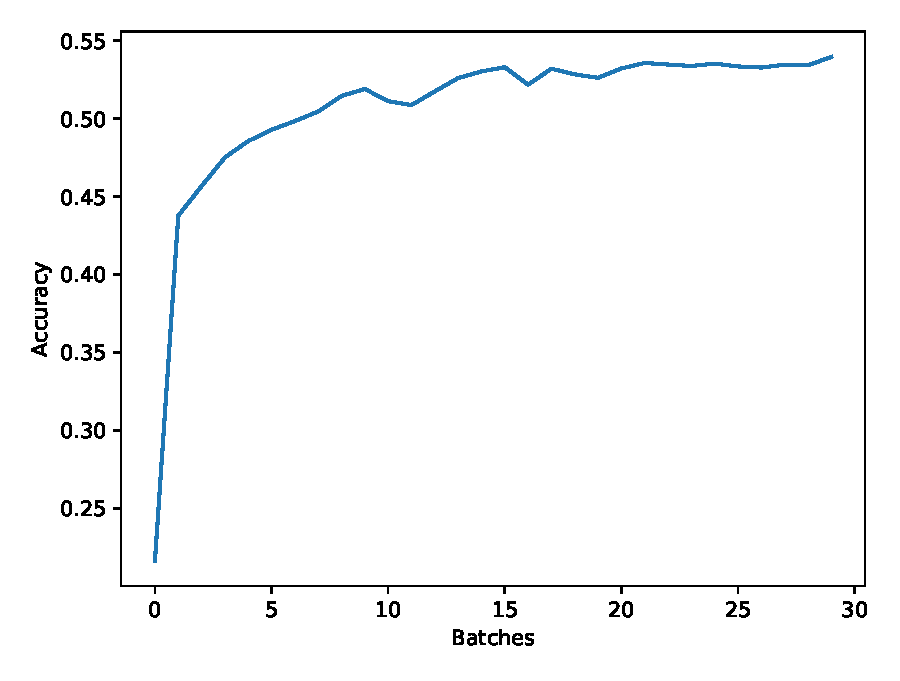
\includegraphics[width=.5\textwidth]{torchAccuracy.eps}}
	\subfloat[]{\includegraphics[width=.5\textwidth]{torchLoss.eps}}
	\caption{Accuracy and loss for the PyTorch implementation of the MLP}
	\label{fig:torchcurves}
\end{figure}
\subsubsection*{Question 2.2}
Using Tanh instead of ELU mainly has drawbacks. The most important one is the problem of vanishing gradients. Since the derivative of Tanh always lies between 0 and 1 (except at identically 0), the gradients attenuate during backpropagation. As a consequence, the shallow layers learn much slower compared to the deeper layers. A possible advantage of Tanh over ELU is that it is zero-centered, meaning that its average output is zero. Zero-centered inputs lead to better training, so a zero-centered activation function is desired. This problem can however be solved by adding batch normalization between layers.
\section{Custom Module: Layer Normalization}
\subsection{Automatic differentiation}
\subsubsection*{Question 3.1}
See the accompanying code
\subsection{Manual implementation of backward pass}
\subsubsection*{Question 3.2}
\begin{enumerate}[label=(\alph*)]
	\item 
	Given that
	$$
	Y_{sj} = \gamma_i\hat{X}_{sj} + \beta_j,
	$$ we will find the required derivatives. 
	\begin{enumerate}[label=(\roman*)]
		\item 
		$$
		\pfrac{L}{\gamma_i} = \sum_{s,j}\pfrac{L}{Y_{sj}}\pfrac{Y_{sj}}{\gamma_i}.
		$$
		But
		$$
		\pfrac{Y_{sj}}{\gamma_i} = \hat{X}_{sj}\delta_{ij},
		$$
		and therefore
		$$
		\pfrac{L}{\gamma_i} = \sum_{s,j}\pfrac{L}{Y_{sj}}\hat{X}_{sj}\delta_{ij} = \sum_s\pfrac{L}{Y_{si}}\hat{X}_{si}.
		$$ In vectorized form, this is equivalent to
		$$
		\pfrac{L}{\b \gamma} = \left(\pfrac{L}{\b Y}\right)^T\hat{\b X}
		$$
		\item
		$$
		\pfrac{L}{\beta_i} = \sum_{s,j}\pfrac{L}{Y_{sj}}\pfrac{Y_{sj}}{\beta_i}.
		$$
		But
		$$
		\pfrac{Y_{sj}}{\beta_i} = \delta_{ij},
		$$
		and therefore
		$$
		\pfrac{L}{\beta_i} = \sum_{s,j}\pfrac{L}{Y_{sj}}\delta_{ij} = \sum_s\pfrac{L}{Y_{si}}.
		$$ In vectorized form, this is equivalent to
		$$
		\pfrac{L}{\b \gamma} = \b 1\pfrac{L}{\b Y}
		$$ where $\b 1$ is the $1 \times S$ ones-vector.
		\item 
		$$
		\pfrac{L}{X_{ri}} = \sum_{s,j}\pfrac{L}{Y_{sj}}\pfrac{Y_{sj}}{X_{ri}} = \sum_{s,j}\pfrac{L}{Y_{sj}}\pfrac{Y_{sj}}{\hat{X}_{sj}}\pfrac{\hat{X}_{sj}}{X_{ri}},
		$$ where we used the fact that $Y_{sj}$ depends only explicitly on $\hat{\b X}$ via $\hat{X}_{sj}$, such that we do not need to write another sum over the elements of $\hat{\b X}$. Notice that $\hat{X}_{sj}$ depends both implicitly and explicitly on $X_{ri}$. Therefore we calculate the total derivative of $\hat{X}_{sj} = f(X_{sj}, \mu_s, \sigma^2_s)$ with respect to $X_{ri}$.
		$$
		\begin{aligned}
		\pfrac{f}{X_{ri}} &= \pfrac{\hat{X}_{sj}}{X_{ri}} + \pfrac{\hat{X}_{sj}}{\mu_s}\pfrac{\mu_s}{X_{ri}} + \pfrac{\hat{X}_{sj}}{\sigma_s^2}\pfrac{\sigma_s^2}{X_{ri}} \\ &= \delta_{rs}\delta_{ij} -\frac{1}{\sqrt{\sigma_s^2 + \epsilon}}\cdot\frac{1}{M}\sum_l\delta_{rs}\delta_{li} - \frac{1}{2}\left(X_{sj} - \mu_s\right)\left(\sigma_s^2 + \epsilon\right)^{-3 / 2}\cdot\frac{2}{M}\sum_l\left(X_{sl} - \mu_s\right)\delta_{rs}\delta_{li} \\ &= \delta_{rs}\delta_{ij} -\frac{\delta_{rs}}{M\sqrt{\sigma_s^2 + \epsilon}}\sum_l\delta_{li} - \frac{\left(\sigma_s^2 + \epsilon\right)^{-3 / 2}}{M}\left(X_{sj} - \mu_s\right)\left(X_{si} - \mu_s\right)\delta_{rs} 
		\end{aligned}
		$$ The remaining expression to find is $\pfrac{Y_{sj}}{\hat{X}_{sj}}$:
		$$
		\pfrac{Y_{sj}}{\hat{X}_{sj}} = \gamma_j
		$$ We can now combine the found expressions to calculate the required derivative.
		$$
		\begin{aligned}
		\pfrac{L}{X_{ri}} &= \sum_{s,j}\pfrac{L}{Y_{sj}}\gamma_j\left[\delta_{rs}\delta_{ij} -\frac{\delta_{rs}}{M\sqrt{\sigma_s^2 + \epsilon}}\sum_l\delta_{li} - \frac{\left(\sigma_s^2 + \epsilon\right)^{-3 / 2}}{M}\left(X_{sj} - \mu_s\right)\left(X_{si} - \mu_s\right)\delta_{rs}\right] \\ &= \pfrac{L}{Y_{ri}}\gamma_i - \sum_{l,j}\pfrac{L}{Y_{rj}}\frac{\gamma_j\delta_{li}}{M\sqrt{\sigma_r^2 + \epsilon}} - \sum_j\pfrac{L}{Y_{rj}}\frac{\gamma_j\left(\sigma_r^2 + \epsilon\right)^{-3 / 2}}{M}\left(X_{rj} - \mu_r\right)\left(X_{ri} - \mu_r\right) \\ &= \pfrac{L}{Y_{ri}}\gamma_i - \frac{1}{M\sqrt{\sigma_r^2 + \epsilon}}\sum_{l,j}\pfrac{L}{Y_{rj}}\gamma_j\delta_{li} - \frac{\left(\sigma_r^2 + \epsilon\right)^{-3 / 2}}{M}\hat{X}_{ri}\sum_j\pfrac{L}{Y_{rj}}\gamma_j\hat{X}_{rj}
		\end{aligned}
		$$
	\end{enumerate}
	\item
	See the accompanying code.
	\item
	Likewise, the implementation can be found in the attached python files.
	\item
	Batch normalization speeds up training by normalizing neuron inputs with the batch statistics \cite{ioffe2015batch}. This is useful when the batch size is significant, because the accuracy of the mean and variance estimates increases with the batch size. This approach can not be applied when training must be done with single-sample batches, or when training an RNN. For that reason, layer normalization was introduced \cite{ba2016layer}. It has the same effect of speeding up training, and has proved very effective for RNNs. However, it does not performs as well on image classification tasks, as discussed in the lecture.
	
	Now we will discuss the performance of the two methods for different batch sizes. For small sizes, batch normalization will result in less accurate statistics, and therefore will not be as effective. For large batch sizes, batch normalization will yield very accurate statistics and therefore the method will be very effective in generating normally distributed activations. Like discussed before, in layer normalization statistics are computed over the feature dimension. This gives a set of statistics for each sample in the batch, and the performance of layer normalization is therefore independent of batch size. 
\end{enumerate}
\bibliographystyle{abbrv}
\bibliography{references.bib}
\end{document}
